% 原书 p.99–p.100（PDF p.107–p.108）
% 第 4 章 4.3 节（续）：邻域定理

% >>> p107
\begin{wproof}[定理 4.3.3 的证明]
  取 $U$ 为 $0_L\subset T^*L$ 的邻域、$V\subset M$ 为 $L\subset M$ 的邻域（来自
  定理 4.3.4），考虑映射 $\psi\colon U\to V$，定义为
  \begin{equation*}
    \psi(q,p):=\exp_q\bigl(\beta^{-1}(p)\bigr)
    \quad\text{对任意}\ (q,p)\in U,
  \end{equation*}
  其中 $\beta$ 是 (4.24) 中定义的映射。必要时可把 $U$ 与 $V$ 取得更小，使 $\psi$ 是
  微分同胚。我们要验证 $\psi^*\omega$ 与 $\omega_{\mathrm{can}}$ 在 $U$ 中的 $0_L$ 上
  相等，从而可以应用引理 4.3.1。

  记 $(x_i,y_i^*)\in T_{(q,0)}T^*L\simeq T_qL\oplus T_q^*L$，其中 $x_i\in T_qL$，
  $y_i^*\in T_q^*L$，$i=1,2$。则
  \begin{equation*}
    \begin{aligned}
      (\psi^*\omega)_{(q,0)}\bigl((x_1,y_1^*),(x_2,y_2^*)\bigr)
      &=\omega_{(q,0)}\bigl(\dd\psi(x_1,y_1^*),\dd\psi(x_2,y_2^*)\bigr)\\
      &=\omega_{(q,0)}\bigl(x_1+\beta^{-1}(y_1^*),x_2+\beta^{-1}(y_2^*)\bigr)\\
      &=\omega_{(q,0)}\bigl(x_1,\beta^{-1}(y_2^*)\bigr)
      +\omega_{(q,0)}\bigl(\beta^{-1}(y_1^*),x_2\bigr)\\
      &=-\omega_{(q,0)}\bigl(\beta^{-1}(y_2^*),x_1\bigr)
      +\omega_{(q,0)}\bigl(\beta^{-1}(y_1^*),x_2\bigr)\\
      &=-y_2^*(x_1)+y_1^*(x_2).
    \end{aligned}
  \end{equation*}
  与此同时，在 $(q,0)$ 附近的局部坐标卡中可直接计算
  \begin{equation*}
    \omega_{\mathrm{can}}\bigl((x_1,y_1^*),(x_2,y_2^*)\bigr)
    =y_1^*(x_2)-y_2^*(x_1).
  \end{equation*}
  证毕。
\end{wproof}
% [Tutor Note: 含糊点拨——「ψ 是微分同胚」是取足够小的 U、V 保证的：指数映射在零截面
% 附近是局部微分同胚，再复合 β^{-1}。计算中 dψ(x_i,y_i^*) = x_i + β^{-1}(y_i^*) 用到
% 分解 T_{(q,0)}T^*L ≅ T_qL ⊕ T_q^*L，以及 exp_q 在 0 处的微分在 T_qL 方向上为恒等、
% 在法方向上对应 β^{-1}。最后一步 ω(x, β^{-1}(y^*)) = y^*(x) 是定义 β(v) = ω(v,−)
% 的直接改写；若把 β 的符号约定改成 −ω(v,−)，这一串等式会整体变号，与 ω_can 的比较
% 也随之改变，核对时以此为准。]

类似地，对切触流形我们有 Legendre 邻域定理。

\begin{wexer}{4.3.1}
  设 $(M,\xi=\ker\alpha)$ 是切触流形，$L\subset M$ 是勒让德子流形。则存在 $L$ 在
  $M$ 中的邻域 $U$、$0_L\times\{0\}$ 在 $T^*L\times\R$ 中的邻域 $V$，以及微分同胚
  $\varphi\colon V\to U$，使得 $\varphi^*\alpha=\lambda_{\mathrm{can}}+\dd t$，其中
  $t$ 是 $\R$-坐标。这里 $T^*L\times\R$ 是切触流形，其切触形式为
  $\lambda_{\mathrm{can}}+\dd t$，其中 $\lambda_{\mathrm{can}}$ 是由
  $\sum_{i=1}^n p_i\,\dd q_i$ 局部定义的典范 $1$-形式。
\end{wexer}

下面是（辛）Weinstein 邻域定理的一个应用。

\begin{wexam}{4.3.2}
  回忆注 1.6.2 中我们证明了：对任意乘积辛流形
  $(M\times M,\pi_1^*\omega-\pi_2^*\omega)$，对角线 $\Delta\subset M\times M$ 是
  拉格朗日子流形。于是由定理 4.3.3，$\Delta$ 在 $M\times M$ 中的邻域 $U(\Delta)$
  辛同胚于零截面 $0_M\subset T^*M$ 的邻域 $V(0_M)$。

  一般地，我们可以把 $\Symp(M,\omega)$ 中恒等映射的 $C^1$-邻域与 $M$ 上闭 $1$-形式
  向量空间中零点的 $C^1$-邻域等同起来。

  设 $f\in\Symp(M,\omega)$ 与恒等映射 $C^1$-接近，使得 $\mathrm{graph}(f)$ 落在
  对角线 $U(\Delta)$ 的 $C^1$-邻域中（见图 4.6）。由例 1.6.2，$\mathrm{graph}(f)$
  是 $(M\times M,\pi_1^*\omega-\pi_2^*\omega)$ 中的拉格朗日子流形。于是由定理 4.3.3，
  它可以等同于零截面 $0_M$ 的 $C^1$-邻域中的一个拉格朗日子流形，记作
% >>> p108
  $V\subset T^*M$，其中包含 $1$-形式的图像。由例 1.6.3，它必来自一个闭
  $1$-形式。\hfill$//$
\end{wexam}
% [Tutor Note: 含糊点拨——例 4.3.2 的要点是把 Symp(M,ω) 在恒等映射附近的局部结构
% 「线性化」为 M 上闭 1-形式的向量空间：f ↦ graph(f) ↦ 对应的闭 1-形式。全局地，
% 闭 1-形式模去恰当 1-形式（即取通量）刻画的正是 Symp(M,ω) 相对于 Ham(M,ω) 的局部
% 结构，在 M 紧时可由 H^1(M;R) 检测。这一步依赖三件事：Δ 是拉格朗日子流形
% （注 1.6.2）、graph(f) 是拉格朗日子流形（例 1.6.2）、以及 T^*M 中零截面附近的
% 拉格朗日子流形都是某个闭 1-形式的图像（例 1.6.3）。]

\begin{figure}[htbp]
  \centering
  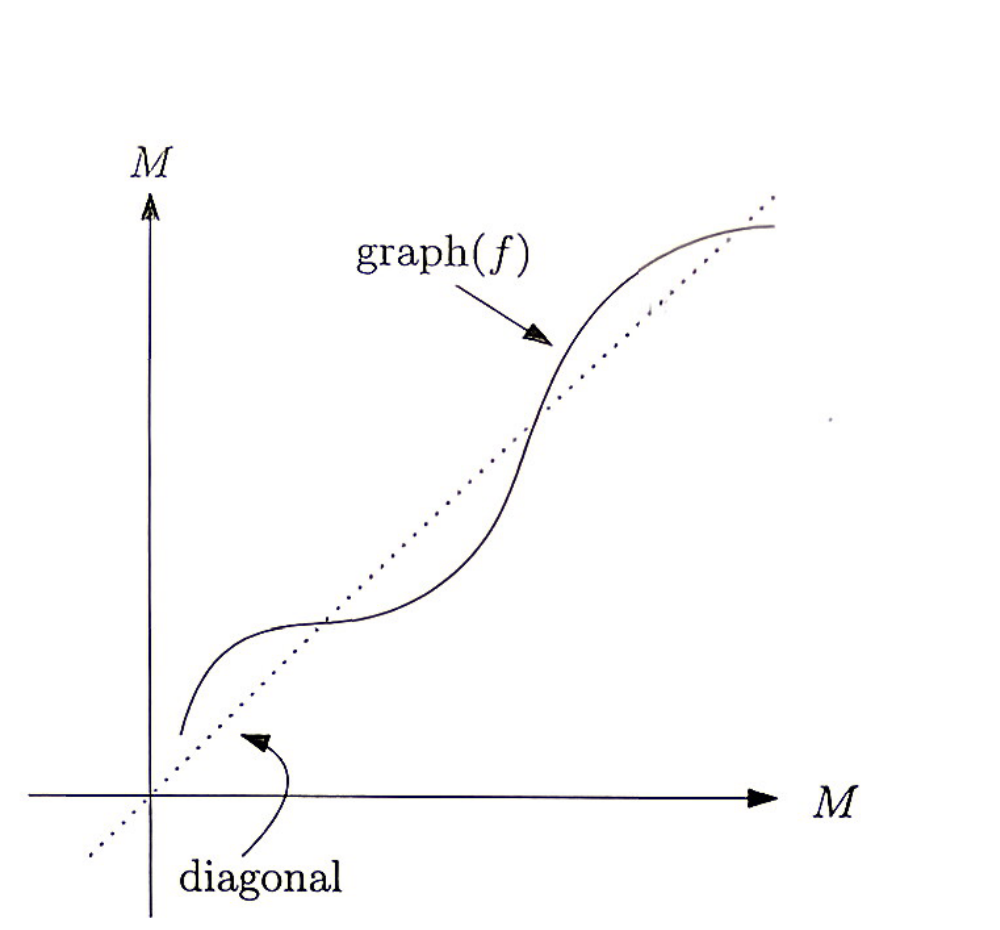
\includegraphics[width=0.55\linewidth]{figures/fig_p108_1.png}
  \caption*{图 4.6\quad 乘积流形中 $f$ 的图像（原书 p.100, Figure 4.6；PDF p.108）}
\end{figure}

最后，为结束本节，我们来给出引理 4.3.1 的证明。

\begin{wproof}[引理 4.3.1 的证明]
  从一条观察开始：如下线性形变
  \begin{equation*}
    \omega_t=(1-t)\omega_0+t\omega_1
  \end{equation*}
  是 $M$ 上的一族光滑闭 $2$-形式，尽管它们未必非退化。但在 $TM|_Q$ 上，
  $\omega_t=\omega_0$ 对任意 $t$ 都非退化。因此存在 $Q$ 的一个邻域，使 $\omega_t$
  在其上非退化。

  让我们应用定理 4.3.4，从 $Q$ 的邻域过渡到其法丛 $NQ\subset TM$。考虑 $NQ$ 上的
  指数映射，它给出从 $NQ$ 中 $0_Q$ 的开邻域 $U$ 到 $M$ 中 $Q$ 的开邻域的微分同胚。
  令 $V=\exp(U)$，我们可以定义 $\varphi_t\colon V\to V$ 为
  $\varphi_t(\exp(q,v)):=\exp(q,tv)$，对任意 $(q,v)\in V$。则 $\varphi_t$ 对
  $t>0$ 是微分同胚。注意当 $t=0$ 时 $\varphi_0(V)\subset Q$，故
  $\varphi_0^*(\omega_1-\omega_0)=0$；而当 $t=1$ 时 $\varphi_1=\mathbf 1$，故
  $\varphi_1^*(\omega_1-\omega_0)=\omega_1-\omega_0$。设 $X_t$ 为流 $\varphi_t$ 的
  向量场，则
  \begin{equation*}
    \begin{aligned}
      \omega_1-\omega_0
      &=\int_0^1\frac{\dd}{\dd t}\varphi_t^*(\omega_1-\omega_0)\,\dd t\\
      &=\int_0^1\varphi_t^*\bigl(\mathcal L_{X_t}(\omega_1-\omega_0)\bigr)\,\dd t\\
      &=\int_0^1\varphi_t^*\dd\bigl(\iota_{X_t}(\omega_1-\omega_0)\bigr)\,\dd t\\
      &=\dd\Bigl(\int_0^1\varphi_t^*\bigl(\iota_{X_t}(\omega_1-\omega_0)\bigr)\Bigr)
      \,\dd t.
    \end{aligned}
  \end{equation*}
  % [Tutor Note: 原文疑误——原文 p.100 末式把 dt 排在右括号之外（即
  % = d(∫_0^1 φ_t^*(ι_{X_t}(ω_1−ω_0))) dt），显系笔误。按定义应有
  % ω_1−ω_0 = ∫_0^1 (d/dt)φ_t^*(ω_1−ω_0) dt
  %         = ∫_0^1 φ_t^* d(ι_{X_t}(ω_1−ω_0)) dt
  %         = d(∫_0^1 φ_t^*(ι_{X_t}(ω_1−ω_0)) dt)，
  % 故 dt 应在积分号内、右括号内。译文保留原文写法，详见 qsg/notes/review_ch04.md。]

  于是我们得到 $NQ$ 上的一个 $1$-形式 $\sigma$，使得 $\dd\sigma=\omega_1-\omega_0$，
  且对一切 $q\in Q$ 有 $\sigma|_{T_qNQ}=0$。最后，我们可以对
  $\omega_t=\omega_0+t\,\dd\sigma$ 运行 Moser 论证，其中 $t\sigma$ 正是所需的一族
  $1$-形式。
  % [Tutor Note: 原文疑误（表述含混）——若取 ω_t = ω_0 + t dσ，则按 (4.1) 所需的
  % 1-形式族应取 σ_t ≡ σ（固定），而不是 tσ；作者此处应是想说明「ω_t − ω_0 = d(tσ)」，
  % 即 tσ 是 ω_t − ω_0 的一族原像。另原文下一句「对任意 (q,v) ∈ V」中的 V 应为 U
  % （因为 exp 只定义在 U 上，且需 (q,tv) ∈ U）。两处均照原文译出，详见
  % qsg/notes/review_ch04.md。]
\end{wproof}
